%% We use `subfiles' package
\documentclass[preamble.tex]{subfiles}
\begin{document}

\clearpage

\chapter{Loop representation: The Loop Language}
\label{ch:Loops}

\LiveFusion at the top level is a library of high level array combinators. Most of these conceptually represent a loop. Indeed, the user of the library can reason about the individual combinators as loops and consider the result of each to be an array.

However, when running the user's program, we are aiming to perform the required operations in as few loops as possible\footnote{This may increase register pressure. However, unless register spilling poses a problem in the future we favour the decreased memory traffic which is attained by array fusion.}. \todo{We have discussed the conditions for fusible combinators in Section ... In general, however...} Subject to certain restrictions, two combinators in \LiveFusion are fusible when the output array \*produced* by one combinator is \*consumed* as input by another combinator one element at a time from beginning to end.

In the \LiveFusion AST discussed in the previous chapter, this relationship is usually seen between a child node (the producer) and its parent node (the consumer). This is not true for \*random access* combinators like @backpermute@ which we discuss separately\todo{in Section }.

\todo{How do we know whether two combinators can be fused?}Intuitively, two combinators can be fused whenever one could write a loop by hand which would give the same final result for the same input as the two separate loops would.
%We need a way to programmatically determine whether a given pair of combinators can be replace with a semantically equivalent loop.

%The focus of this chapter is to establish the requirements for fusible combinators and define a loop representation to which such fusible combinators can be mapped.
The focus of this chapter is to establish a common loop representation to which fusible combinators can be mapped.

In the following sections we will look more closely at what a loop really is and then present the core of our fusion optimisation.


\clearpage

\section{Anatomy of a loop}
\label{sec:anatomy}

Despite the purely functional, combinatorial interface to the library, looking at a loop in a procedural way is the approach I have opted for in the middle layer of the system. It is represented by the \Loop language.\iloop

The loops \LiveFusion generates can be viewed as similar to those one might write in an Assembly language. It uses labelled basic blocks and has explicit control flow using @goto@ statements\footnote{The formal grammar of the \Loop language is introduced later in the chapter. It is presented in Figure \ref{fig:Loop-grammar} on \pageref{fig:Loop-grammar}}.

However, as we will see later, they are often even more structured than loops in \C and other mainstream procedural languages. As such I urge the reader to think of them as being high-level and treat the explicit control flow as implementation details.

%The downside, however, is that our loop relies on @goto@-like statements whose use is almost always considered bad practice in modern software engineering.

Without further delaying the discussion of the matter we will now look are the structure of a typical @for@ loop in a language like \C in an attempt to shape our own loop structure.


\subsection{Structure of a \code{for} loop}

Consider the following fragment of a \C program that creates a new array @ys@, by applying some function @f@ to those elements of array @xs@ that satisfy some predicate function @p@ (in \Haskell this could be expressed as @ys = (filter p . map f) xs)@):

\begin{ccode}[numbers=left]
double *ys = malloc(len * sizeof(double)); // result array
int i = 0;                                 // output index
for(int i = 0; i < len; i++) {
    if(p(xs[i])) {
        ys[j] = f (xs[i]);
        j++;
    }
}
ys = realloc(ys, j * sizeof(double));
\end{ccode}

A @for@ loop in \C has four sections:

\begin{enumerate}
\halfspacing
\item \*initialisation* section (@i = 0@),
\item \*guard* section (@i < len@),
\item the main \*body* (@if(){ ... }@), and finally
\item the \*update* section (@i++@).
\end{enumerate}

Compared to free-formed @while@ loops which only have a @guard@ and a @body@, the @for@ loops are already much more structured.

However, as we will now show, further structural elements could be introduced which will ultimately assist us when composing loops from array combinators.


\subsubsection{Initialisation}

The very first observation to make is that both the result array @ys@ and the output index @j@ were declared and initialised outside the @for@ loop.

In pursuit of a more structured and composable approach to looping all statements executed \*once* before the loop begins are placed in the \[init] basic block of the loop.

The initialisation code corresponds to the following in the \Loop language:

\begin{loopcode}
init:
  let len = arrayLength xs
  let ys = newArray len
  let i = 0
  let j = 0
  goto guard
\end{loopcode}


\subsubsection{Guard}

The @guard@ of a @for@ loop corresponds to a \[guard] block of in the \Loop language. It can contain arbitrary statements but usually contains at least one @unless@ statement:

\begin{loopcode}
guard:
  unless i < len | done
  goto body
\end{loopcode}

The @guard@ \*statement* transfers the control to a different block if the condition is \*false* (to \[done] in this case).


\subsubsection{Update}

The @update@ equivalent of a @for@ loop in the \Loop language is the basic block called \[bottom]:

\begin{loopcode}
bottom:
  i := i + 1
  goto guard
\end{loopcode}

The block so called because it is executed \*unconditionally* at the end of each iteration.

As seen in the code above \Loop language supports destructive updates through using @assignment@ (@:=@).


\subsubsection{Finalisation}

The @filter@ results in a shorter array in the general case. Hence, after the @for@ loop finishes, the resulting array is \texttt{realloc}'ated to free the unused memory (in practice the array is unlikely to be copied).

This is one of the use cases for what is called a \[done] block of the loop:\todo{As we will see later it is not only useful for trimming and returning the final array but also for scheduling other loops such as in @append@ combinator.}.

\begin{loopcode}
done:
  let result = sliceArray ys j   -- resize to length j
  return result
\end{loopcode}

As seen from the code, every loop has a result which it returns explicitly.


\subsection{``Dissecting loop bodies''}

We will now attempt to categorise the types of operations that all belong to the bodies of conventional @for@ and @while@ loops.

\subsubsection{Reading and writing arrays}

Line 5 of the @for@ presented above (@ys[j] = f (xs[i]);@) is actually doing three things:
\begin{enumerate}
\halfspacing
\item \*reading* an element from array @xs@,
\item \*producing* a new element by applying @f@ to it, and
\item \*writing* the new element into array @ys@.
\end{enumerate}

Consider, however, that we are trying to devise a loop representation for an application of fusion. When several combinators are fused into a single loop and produce no intermediate arrays, such reading and writing only happens at the beginning and at the end of a combinator pipeline.

Hence we want to separate the notion of \*producing* a new element from the fact that it came from an array, a list or just another computation. Likewise, we do not need to be concerned with how the new element is going to be consumed. It may or may not be written into a new array. It may or may not be used by a consuming combinator. However, it should not up to an individual combinator to decide.

In fact, an element may not even be produced as we discuss next.


\subsubsection{Skip producing an element}

Combinators like @filter@ may not produce a new element in every iteration. This was the case with the example above where only elements satisfying predicate @p@ were used. The \*guard* of the @if@ was serving as a predicate check which its body was the code that produced the element.

The \Loop language attempts to be more precise about where the element is produced. The code is split across two blocks: \[body] and \[yield]:

\begin{loopcode}
body:
  let x = readArray xs i
  unless (p x) | bottom  -- end iteration if the predicate is not satified
  let y = f x
  goto yield

yield:
  writeArray ys j y
  j := j + 1
  goto bottom
\end{loopcode}

The \[body] block deals with all the code that is concerned with producing an element, however an element is known to have been produced only if it the control reaches the \[yield] block.

This allows us to make assumptions about the behaviour of a loop without knowing what the loop is doing internally. As we will see later, the code that introduces @writeArray@ statements into the loop is oblivious to how the element has been produced. It knows that an element has definitely been produced if the control enters the \[yield] block.


\subsection{The complete example}

We have now constructed a complete loop in the internal \Loop language which corresponds to the \C code at the beginning of the section. The \C code in turn corresponds to \Haskell program @ys = (map f . filter p) xs@.

Both the original program and the resulting loop are given in Figure~\ref{fig:MapFilter}.


\begin{figure}

\begin{subfigure}{.45\textwidth}
\begin{loopcode}
init:
  let len = arrayLength xs
  let ys = newArray len
  let i = 0
  let j = 0
  goto guard

guard:
  unless i < len | done
  goto body

body:
  let x = readArray xs i
  unless (p x) | bottom
  let y = f x
  goto yield

yield:
  writeArray ys j y
  j := j + 1
  goto bottom

bottom:
  i := i + 1
  goto guard

done:
  let result = sliceArray ys j
  return result
\end{loopcode}
\end{subfigure}%
%
\begin{subfigure}[right]{.55\textwidth}
\begin{ccode}
double *ys = malloc(len * sizeof(double));
int i = 0;
for(int i = 0; i < len; i++) {
    if(p(xs[i])) {
        ys[j] = f (xs[i]);
        j++;
    }
}
ys = realloc(ys, j * sizeof(double));
\end{ccode}
\end{subfigure}

\caption{Computation \code{ys = (map f . filter p) xs} in \C (right) and internal \Loop language (left).}
\label{fig:MapFilter}
\end{figure}


\subsection{Summary of Loop structure}
\label{sec:anatomy-summary}

In summary the common loop structure to be used throughout this chapter is comprised of the following 6 loop section (represented by basic blocks in the \Loop language):\iblock
\begin{enumerate}
\item \[init] block is the main entry into the loop and contains statements which need to execute only once for the whole loop. New array allocation, index and length variable initialisation all belong here.
\item \[guard] block performs looping condition tests before every iteration of the loop.
\item \[body] block contains all statements concerned with reading arrays and computing elements.
\item \[yield] block is entered only if a \*new element* has been produced by the loop in the current iteration. It is not entered is the loop's logic has skipped to the next iteration without producing an element (e.g. in @filter@ combinator). This is the place to write the produced element in the resulting array if required.
\item \[bottom] block is entered unconditionally at the end of every iteration whether of not an element has been produced. It roughly corresponds to the \*update* section of a @for@ loop in procedural languages. Uses beyond simple index advancement will be seen later in this chapter.
\item \[done] block performs any remaining operations after the loop has finished. In particular it returns the final result from the loop. Unlike the loops in the majority of procedural languages the @return@ of a value from a loop in the \Loop language is explicit.
\end{enumerate}


\clearpage

\section{The \Loop language more formally}
\label{sec:The-Loop-language}
\iloop

In summary we have used the following features of the \Loop language in the previous example:
\begin{enumerate}
\halfspacing
\item New variable binding (@i = 0@)
\item Variable assignment (@i := i + 1@)
\item Explicit control transfer (@goto body@)
\item Conditional control transfer (@guard i < len | done@)
\item Returning values from loop (@return ys'@)
\item A number of built-in array primitives: (@newArray@, @readArray@, @writeArray@, @arrayLength@ and @sliceArray@).
\end{enumerate}

All of the above are \*statements*, which are grouped into labelled \*basic blocks*.\iblock

The grammar of the \Loop language is presented formally in Figure~\ref{fig:Loop-grammar}. The syntax seen in the examples throughout this thesis is the same as used by the pretty printer for the language and it faithfully\footnote{I have taken the liberty of rewriting operators in infix notation and omitting explicit literal conversions such as \code{fromInteger 1}.} reproduces the internal representation of \Loop programs. 

\begin{figure}[htpb]
\subfile{loop-grammar}
\caption{\label{fig:Loop-grammar}Grammar of \Loop language.}
\end{figure}
\todo{Put the footnotetext on the same page where the grammar ends up}
\footnotetext{For improved readability the unique integers are replaced with meaningful names in the code listings. \*(Footnote for listing \ref{fig:Loop-grammar})*}

If the grammar is studied more carefully one would note two each basic block may have multiple associated labels. As we will see in the next section this is a vital feature of the language which allows for easy fusion of loops.

We also note that each label and variable in the language is postfixed with a unique value which has so far been omitted from the listings.

Being a flexible assembly-style language the \Loop language is not limited by the basic block structure discussed in Section~\ref{sec:anatomy} and summarised in Section~\ref{sec:anatomy-summary}. However, as seen in the rest of this chapter this structure has proven to be a useful common base for many types of arrays combinators. Thus we assume this to be the common pattern of using the \Loop language.

Semantically, the \Loop language does not presume a fixed order of evaluating @let@ bound variables. However, all statements affecting control flow (@goto@, @unless@, @if@) are executed in the order they appear in the block.

Lastly, the new value of assigned variables ($\coleq$) is not available until the next block the control is transferred to. This is an implementation side-effect of the \*liveness analysis* pass (Section~\ref{sec:Liveness-analysis}) which however is helpful in implementing fused loops.


\clearpage

\section{Fused loops generation}
\label{sec:loop-generation}

In the previous section we have seen the first example of the \Loop EDSL which computed at @filter@ of an array followed by a @map@. We have also identified five main \*sections* of a loop, represented by \*basic blocks* in the \Loop language: \[init], \[guard], \[body], \[yield], \[bottom] and \[done].

We shall revisit the example from the previous section and introduce the process by which a \Loop is generated.

This time we extend the example with specific functions passed to @map@ and @filter@ combinators. The function @toPercentages@ shown on Figure~\ref{fig:toPercentages} (left) converts an array fractions to their percentage equivalents, filtering out those below $0.01$ (or $1\%$).

\begin{figure}
\begin{subfigure}{.65\textwidth}
\begin{hscode}
toPercentages :: Array Double -> Array Double
toPercentages fractions
  = let significant = filter (>=. 0.01) fractions
        percents    = map (* 100) significant
    in  percents
\end{hscode}
\end{subfigure}%
%
%\begin{subfigure}{.3\textwidth}
%  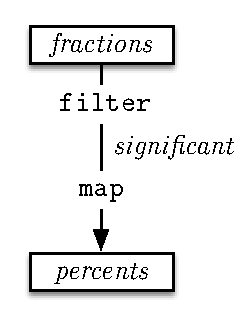
\includegraphics[height=12em]{img/toPercentages-flow}
%\end{subfigure}
%
\begin{subfigure}{.35\textwidth}
  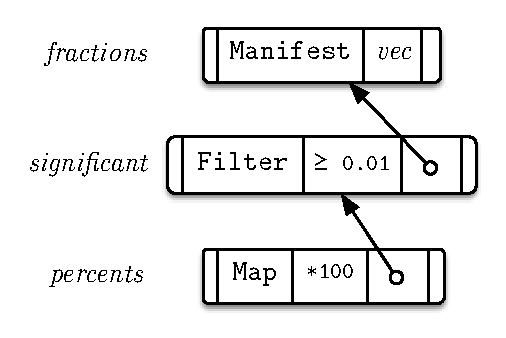
\includegraphics[height=10em]{img/toPercentages-ast}
\end{subfigure}
\caption{\code{toPercentages} function (left) and its \LiveFusion AST (right).}
\label{fig:toPercentages}
\end{figure}



\subsection{Start with an AST}

The @toPercentages@ function internally uses a pipeline of to combinators: the output array of @filter@ (@significant@) becomes the input array of @map@. Remembering that @Array Double@ is the type synonym for @AST (Vector Double)@, each combinator constructs a node in an AST representing a \*delayed array computation*.

It is impossible possible to know statically whether the input @fraction@ array is computed by a long pipeline of combinators or is a @Manifest@ array stored in memory. Likewise, it is not known before the runtime if the resulting @percents@ array is consumed by another combinator and the pipeline of delayed operation will continue to grow after @toPercentages@ function returns.

For the purposes of illustration we will assume that the @toPercentagee@ function is called with a @Manifest@ array as argument and the result is immediately \*forced* to be computed (e.g. to be printed out or to be consumed in a random access fashion).

In this case the AST shown on Figure~\ref{fig:toPercentages} (right) is constructed and \*forced* to a @Manifest@ array at the runtime of the program:

\begin{hscode}[mathescape]
-- AST that may be generated for a call to toPercentages
ast :: AST (Vector Double)
ast = force $\dol$ Map (* 100) $\dol$ Filter (>=. 0.01) $\dol$ Manifest vec

-- LiveFusion library functions
force :: Elt a => AST (Vector a) -> AST (Vector a)
force = Manifest . evalArrayAST

evalArrayAST :: Elt a => AST (Vector a) -> Vector a
evalArrayAST = $...\ compile\ AST\ and\ compute\ result ...$
\end{hscode}

The three fusible combinators represented by @Manifest@, @Filter@ and @Map@ AST nodes are followed by the call to an evaluator, which processes them individually as shown next.
% After sharing recovery each AST node (or rather ASG node) is assigned a unique value


\subsection{Generate loops for individual combinatos}

In order to generate the \Loop code for an AST of combinators, the evaluator first processes them individually. For each combinator it populates the parts of the loop that were identified in Section~\ref{sec:anatomy}. It does so by inserting new statements into the appropriate basic blocks of a loop template comprising of thus instantiating the loop template.

\subfile{lst-toPercentages-loops}

The left of Figure~\ref{fig:toPercentages-loops} shows the loops generated for the individual combinators. It is implicitly referenced in the following discussion.

All variables and labels introduced by a particular combinator are given a unique identifier. In listings these are: \*mfst* (short for \*Manifest*), \*map* or \*filt*.

Internally however, the library uses unique integers to distinguish between similarly named variables and labels belonging to different combinators (e.g. @body_2@ and @elt_3@). This not only avoids variable name clashes, but as we will see later, enables communication between combinators through naming conventions.


\subsubsection{Iteration over a \code{Manifest} array}

Recalling that the @Manifest@ combinator is the only combinator in the pipeline that holds a reference to the physical array, its loop does nothing more than to read the array \|arr_mfst| element by element.

It is worth noting that the array is not @let@-bound in any of the blocks. This is due to the fact that the array is an \*argument* to the loop and is passed from the running program when the computation is finally ready to be performed (code generation and loading are discussed in Chapter~\ref{ch:Code-Generation}).

The combinator introduces a length variable \|len_mfst| and a counter variable \|ix_mfst|. It also has its own set of basic blocks \|init_mfst| ... \|done_mfst|.

The result of array read is placed in \|elt_mfst| variable.


\subsubsection{Filter and variable naming conventions}

In the loop representing @filter@ code all bound variables and label names are identified by \*filt*.

One will notice the absence of @goto@s in the generated \Loop code. The filter relies to the underlying combinators to provide the valid control flow.

As discussed previously in Section~\ref{sec:Scalar-language} it is essential performance that the user functions parametrising combinators be inlined in the generated code. In case of a @filter@ the predicate function $(\geq 0.01)$ has been inlined as the predicate expression to the @unless@ statement.

Since the length output array of @filter@ may be different from the length of input, a new counter variable \|ix_filt| is introduced.

The length variable \|len_filt| representing the \*upper bound* on the length of output array is rebound to be the same as \|len_mfst| of @Manifest@ combinator. Similarly, the resulting element of \|elt_filt| is rebound to be \|elt_mfst| -- the output of @Manifest@ from the same iteration.

These are examples of \*naming conventions* used to facilitate communication between consecutive combinators in a pipeline. In particular the following are always true for a combinator with identified \*id*:

\begin{itemize}
\halfspacing
\item Variable \|elt_id| contains the value of produced element at every iteration
\item Variable \|len_id| contains the upper bound on the length of the output array
\item Variable \|ix_id| contains the index of the element being produced.
\end{itemize}

Rebinding the three variables in every combinator ensures that this information is \*propagated* upwards through the pipeline of combinators. In particular, the @filter@ only required to know the \*id* of @Manifest@ combinator below it to infer these variables.

\begin{bluebox}
By design the combinators know the unique identifiers of the combinators they are referencing and nothing else.
\end{bluebox}


\subsubsection{Map}

Populating the loop with @map@-specific statements is straight-forward.

Since the length \|len_map| and the iteration index \|ix_map| are always the same as those of the input array (output of @filter@), they are simply rebound. This means that @Manifest@ combinator uses one index, while both @filter@ and @map@ are using another. This supports the \*rate*-changing\irate nature of @filter@.

Again, the user specified function $(* 100)$ is inlined to facilitate generation of fast code.


\subsubsection{Physical array creation}

For the @toPercentages@ example we said the pipeline of combinators will be forced to a @Manifest@ array immediately after the @map@.

The statements required to allocate, populate, slice and return the new array are self-explanatory.

It is worthy of note that the design decision to transfer control to \[yield] block whenever an element is produced has made it very easy to introduce the array write.



\subsection{Merging loops}

We have given the \Loop language representations for @Manifest@, @map@ and @filter@ combinators as well as the code that writes out physical arrays.

In order a create one succinct loop, these individual loops are merged into one loop as they are being created. Each combinator has access to the loop composed by all of the combinators below it. For example, when fusing the @map@ the cumulative loop of both @filter@ and @Manifest@ is available for it to be merged with.

For combinators as simple as @map@ and @filter@ merging loops means to simply merge the statements of the corresponding blocks blocks in no particular order.

As seen from the final loop on Figure~\ref{fig:toPercentages-loops} (right), not only the block statement lists have been merged together, but also the block labels: each block can now be identified by any of the three identifiers (\*mfst*, \*filt*, \*map*).

This is done in order to support fusing complex ASTs with lots of shared nodes. The benefit of this may appear much clearer when we introduce nested combinators\todo{in Section}.
\todo{Elaborate.}


\subsubsection{Managing label sets with \name{AliasMap}}

In order to achieve the flexibility of having multiple labels associated with the same block I have implemented a new type of associations @Map@ called \name{AliasMap}.

It offers a familiar interface (Listing~\ref{lst:AliasMap-interface}) similar to that of \Haskell's @Data.Map@. The difference is that it allows for a \*set* of keys to be associated with one value. In addition to the usual functions found in @Data.Map@ one will allow to query the map using \*synonyms*. That is, it will produce a given any one keys associated with the value.

The notion of \*key synonyms* is used throughout \name{AliasMap} interface which greatly facilitates managing and merging loops where blocks are associated with multiple labels.

\lstinputlisting[style=haskell, float, caption={\name{AliasMap} interface (partial). \code{Ord k} constraints omitted for brevity.}, label=lst:AliasMap-interface]{listings/AliasMap-interface.hs}


\section{More on \texttt{goto}s}

While the use of @goto@s is considered bad practice in modern software engineering I note several reasons for using them in the \Loop intermediate language:

\begin{itemize}
  \item It is completely hidden from the library user.

  Given a well behaving \Loop code generator the produced code will always be valid if the user program is valid.

  This is akin to using @unsafePerformIO@ and similar within the library internals for performance reasons. They can lead to bad code but with careful use give very noticeable advantages to purely functional programs.

  \item The \Loop language was designed with a pluggable backend in mind.

  It was assumed that assembly-like \Loop language would be easier to connect with any backend.

  Specifically in the \Haskell backend, @goto@ statements are translated to tail-recursive function calls.

  An \LLVM backend is also planned. \LLVM uses very similar notions of \*basic blocks*.

  \item The @goto@ based design was the most flexible and the easiest to implement.

  Nonetheless, this does not prevent the \Loop language from being extended to support a more statically safe programming model.
\end{itemize}



\clearpage

\section{Flat array cominators}

\subsection{Reductions}

\begin{comment}
We have already looked at how the indices maintain the state of the loop between iteration. However, indices, although the most obvious state the loop has, are not the only ones. If we think of standard list combinators that pass partial results with the recursive calls as accumulators, @fold@s and @scan@s immediately come to mind. In practice, declaring and using accumulator variables like this in a loop language is straight-forward and is no differect from declaring and using index variables. They both represtent mutable variables in the loop language.

Suppose that out expressing is `scan (*) 1 xs'. We already know how to generate code for iterating the $xs$ array. It may or may not be a manifest array. We trust that the combinator producing $xs$ has already generated the appropriate code in the loop we are trying to construct.

If @scan@ gets the id of 6 in the pipeline, then we know that it can access its input elements in $elt_{i_6}$, the index of the iteration in $i_6$. Any local variable will also get postfixed with id 6. As such we will declare $f_6 = (*)$ as the reduction function, $acc_6 = 1$ as the mutable accumulator value containing the initial value. Moreover, we will be placing the output element for the current iteration in $elt_{o_6}$.
\end{comment}


\subsection{Zipping}

\begin{comment}
So far the combinator pipelines we have looked at had a list like structure. Each combinator would consume exactly one array and produce another. However, for many programs this is not sufficient. In many cases a combinator takes multiple arrays as input. In general there is no constraint on how a combinator would consume each of those arrays. Some combinators (e.g. @backpermute@) require that one of the passed arrays is random-access, however, some, like @zipWith@ consume two arrays in lock step.

A call to `zipWith (*) xs ys' element-wise multiplies arrays $xs$ and $ys$. Those two arrays may internally be pipelines of combinators. A @zipWith@ combinator is such a common occurence in DPH programs that it would be wasteful not to fuse it with the combinators producing $xs$ and $ys$.

%Two difficulties arrising when fusing @zipWith@ with its children is:
%+ the potential difference in lengths between $xs$ and $ys$, and
%+ the duplicated index counters: one iterating $xs$, and one - $ys$

The loops for $xs$ and $ys$ have been generated independently of each other. They have their own index spaces and their own control flows. Suppose that we get the following tree of combinators to compute:

\begin{hscode}
let xs = map (+10) [1..10]
    ys = map (*3)  [100..110]
in  zipWith (*) xs ys
\end{hscode}

We can easily generate the loops for each of $xs$ and $ys$ the way we described previously. We can then merge all of the blocks together with code multiplying the output elements to form a valid loop computing the desired result:

...code...

**The Problem**

The code generated in the previous step will produce correct results for the specific problem. However, it will not work in the general case. Suppose we introduce a filter into `xs':

\begin{hscode}
let xs = filter odd \$ map (+10) [1..10]
    ys = map (*3)  [100..110]
in  zipWith (*) xs ys
\end{hscode}

While @zipWith@ is supposed to consume elements from $xs$ and $ys$ in a lockstep, producing both those elements will not always happen in the same iteration. $ys$ array does not pose a problem, it is guaranteed to produce one element in each iteration. However, the addition of @filter@ into the equation for $xs$ will mean that the loop for $xs$ may need more than one iteration to produce an element. If the @filter@ skips an element the loop for $ys$ must wait.

**A Solution**

We solve the above problem by first analysing the loops for $xs$, $ys$ and $zs$. A quick check of how we would write the above program in C tells us that we would probably still be able to only an overall loop for $zs$. However, we will likely declare two separate counters for computing $xs$ and $ys$. In fact we may also create a separate *nested* loop for $xs$. We will break out of that loop as soon as we have produced an element that satisfied the @filter@ condition.

We know that the length of $ys$ is fixed and is 10. We also know that the length of $xs$ has the upper bound of 10 but is not known until runtime. Incidentally, @zipWith@ will consume as many elements as $xs$ will produce. We say that $xs$ and @zipWith@ have the same rate. Since @zipWith@ is a direct consumer of $ys$, its loop's body should only ever be exectuted once both have finished.

Let us look at the resulting loops

\begin{loopcode}

----------------- INIT OF OUTER LOOP --------------------
init:
  -- xs
  -- id 0: [1..10]
  len_0 = 10
  i_0 = 0
  -- id 1: map (+10)
  f_1 = (+10)
  -- id 6: filter odd
  p_6 = odd
  i_6 = 0   -- output index of filter

  -- ys
  -- id 2: [100..101]
  len_2 = 10
  i_2 = 0
  -- id 3: map (*3)
  f_3 = (*3)

  -- id 4: zipWith (*)
  f_4 = (*)

  -- Default control flow
  goto guard_0

guard:
  -- Check that we haven't exhausted ys
  pred_2 = i_2 < len_2
  guard pred_2 done

  -- Go to nested loop
  goto guard_0

---------------- BEGIN NESTED LOOP ---------------------
-- Nested loop for xs
guard_0:
  pred_0 = i_0 < len_0
  guard pred_0 done_0

body_0:
  -- xs
  -- id 0: [1..10]
  elt_0 = 1 + i_0
  -- id 1: map (+10)
  elt_1 = f_1 elt_0
  -- id 6: filter odd
  elt_6 = elt_1
  pred_6 = p_6 elt_1
  guard pred_6 bottom_0   -- predicate if false, skip

  -- Default control flow
  goto yield_0

yield_0:
  -- Exit nested loop
  goto guard

bottom_0:
  i_0 := i_0 + 1
  -- Move on to next element in ys

done_0:
  -- We have exhausted all elements in ys
----------------- END NESTED LOOP ------------------------

------------------ CONTINUE OUTER LOOP --------------------


body:
  -- ys
  -- id 2: [100..110]
  elt_2 = 100 + i_2
  -- id 3: map (*3)
  elt_3 = f_3 elt_2

  -- zipWith (*) xs ys
  elt_4 = f_4 elt_1 elt_3

  -- Default control flow
  goto write

write:
  ...
  -- Default control flow
  goto bottom

bottom:
  i_0 = i_0 + 1                     -- goto next iteration
  -- Default control flow
  goto guard

-------------------- BOTTOM OF NESTED LOOP --------------------------------
done:

\end{loopcode}
\end{comment}



\clearpage

\section{Random access combinators}

\subsection{Backpermute}

\subsection{Index}



\clearpage

\section{Array generators: Enumeration and Replication}

\subsection{Segmented array combinators}

Two types

\subsection{Segmented scan}

\subsection{Segmented fold}

\subsection{Segmented replicate}



\clearpage

\section{Interleaved loops}

\subsection{Append}

\subsection{Segmented append}


\IfNotCompilingAll{\bibliography{bib}}

\end{document}
